% ─────────────────────────────────────────────────────────────────────────────
%  Печатная спецификация серии «Школа 1С-инженеров»
%
%  Подключается ключом -H при сборке печатного PDF. Формат, поля и шрифты
%  приходят из metadata.yaml через -V, здесь — всё остальное: гарнитуры
%  кириллицы, интерлиньяж, колонтитулы, шмуцтитулы, кромочные вкладки,
%  рубрики, оформление листингов и метки коротких кодов.
%
%  Канон: docs/style-guide.md, разделы 15–17.
%  Разметку для этих окружений готовит scripts/print-prep.py.
% ─────────────────────────────────────────────────────────────────────────────

% Кириллица в трёх гарнитурах. Без этих трёх строк polyglossia ищет
% кириллицу в латинском шрифте и спотыкается на моноширинном.
\newfontfamily\cyrillicfont{PT Serif}
\newfontfamily\cyrillicfontsf{PT Sans}
\newfontfamily\cyrillicfonttt{PT Mono}
% Программистские лигатуры шрифта склеивают <= и >= в ≤ и ≥. Для книги,
% которая учит набирать код, это подмена: таких знаков на клавиатуре нет.
\setmonofont{PT Mono}

% PT Serif не содержит стрелки «→», а в прозе этих книг она встречается
% сотнями. Берём математическую: в серифном наборе она на месте.
\usepackage{newunicodechar}
\newunicodechar{→}{\ensuremath{\rightarrow}}

% Интерлиньяж: 11 pt на 15,5 pt. Ровно 35 строк в полосе высотой 192 мм.
\linespread{1.14}

% Классическая красная строка вместо отбивки между абзацами.
\setlength{\parindent}{5mm}
\setlength{\parskip}{0pt}

% Микротипографика: подрезка полей. На узкой полосе заметно убирает дыры
% между словами при выключке.
\usepackage{microtype}

\clubpenalty=10000
\widowpenalty=10000
\displaywidowpenalty=10000
\setlength{\emergencystretch}{3em}

% Схемы и код: 10,5 pt при базовом 11 pt.
\usepackage{fancyvrb}
\usepackage{fvextra}
\fvset{fontsize=\small,baselinestretch=0.95}

% Код переносится с висячим отступом — ровно так, как он ведёт себя в EPUB,
% и ровно поэтому канон разрешает коду 72 знака, а схеме только 46.
% Схемы в это окружение не попадают: перенос убил бы их выравнивание.
% Листинг: линейка снизу; верхнюю рисует \codetop, потому что она
% уходит в поле и держит метку.
\DefineVerbatimEnvironment{Code}{Verbatim}{%
  fontsize=\small,baselinestretch=0.95,
  frame=bottomline,framerule=0.8pt,framesep=7pt,
  breaklines=true,breakindent=2em,breakautoindent=false,
  % цепочки через точку — один кусок без пробелов; разрешаем рвать
  % после точки и открывающей скобки, как и в тексте
  breakafter={.(},
  breaksymbolleft={\footnotesize\ensuremath{\hookrightarrow}},
  breaksymbolindentleft=0pt,breaksymbolsepleft=0.6em}

% Схема, таблица, вывод программы — не код. Линеек нет.
\DefineVerbatimEnvironment{Plain}{Verbatim}{fontsize=\small,baselinestretch=0.95}

\usepackage{needspace}
\usepackage{tikz}
\newlength{\marklen}\setlength{\marklen}{16mm}

\newcommand{\warnsign}{%
  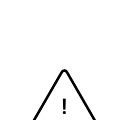
\begin{tikzpicture}[baseline=0pt]
    \draw[line width=0.9pt,rounded corners=0.7mm] (0,0) -- (4.5mm,7.8mm) -- (9mm,0) -- cycle;
    \node[anchor=base] at (4.5mm,1.9mm) {\sffamily\bfseries\footnotesize !};
  \end{tikzpicture}}

% Метка стоит в наружном поле — на нечётной полосе справа, на чётной слева.
% Сторону нельзя взять из \value{page}: материал попадает в вертикальный
% список раньше, чем решится, на какой он полосе. \strictpagecheck узнаёт
% её через метку в .aux — отсюда лишний прогон при первой сборке.
\usepackage{changepage}
\strictpagecheck

% Полная ширина линейки: полоса набора плюс отбивка и метка в поле.
\newlength{\ruleout}
\setlength{\ruleout}{\dimexpr\textwidth+\marginparsep+\marklen\relax}

% Верхняя линейка уходит в поле и держит метку. \needspace не даёт
% разорвать страницу между линейкой, меткой и первыми строками кода.
\newcommand{\markbox}[1]{%
  \raisebox{-\height}[0pt][0pt]{%
    \parbox[t]{\marklen}{\centering\vspace{3pt}#1}}}
\newcommand{\codetop}[1]{%
  \par\addvspace{10pt}\needspace{26mm}\nointerlineskip
  \checkoddpage
  % линейка и метка живут в боксе нулевой ширины: иначе TeX считает
  % выход в поле переполнением строки и засоряет лог
  \noindent\hbox to \textwidth{\hbox to 0pt{%
    \ifoddpage
      \rule[0.6ex]{\ruleout}{0.8pt}%
      \hspace{-\marklen}\markbox{#1}%
    \else
      \hspace{-\dimexpr\marklen+\marginparsep\relax}%
      \rule[0.6ex]{\ruleout}{0.8pt}%
      \hspace{-\ruleout}\markbox{#1}%
    \fi
    \hss}\hfil}%
  \par\nointerlineskip\vspace{-0.6ex}}

\newcommand{\qrmark}[1]{\codetop{\includegraphics[width=14mm]{qr/#1.png}\\[2pt]%
  {\ttfamily\scriptsize #1}}}
\newcommand{\trapmark}{\codetop{\warnsign}}
\newcommand{\plaintop}{\par\addvspace{10pt}\needspace{26mm}\nointerlineskip
  \noindent\rule{\textwidth}{0.8pt}\par\nointerlineskip}
\newcommand{\schemetop}{\par\addvspace{9pt}\needspace{18mm}}

\usepackage{xcolor}
\usepackage{graphicx}
% Метки песочницы живут в наружном поле — том самом, ради которого
% серия и ушла с A5. Полосу набора они не занимают.
\usepackage{marginnote}
\renewcommand*{\marginfont}{\footnotesize}
\usepackage{eso-pic}
\usepackage{etoc}
\usepackage[skins]{tcolorbox}
\usepackage{etoolbox}

% ─── Колонтитулы ─────────────────────────────────────────────────────────────
\usepackage{fancyhdr}
\pagestyle{fancy}
\fancyhf{}
\renewcommand{\chaptermark}[1]{\markboth{#1}{}}
\renewcommand{\sectionmark}[1]{\markright{#1}{}}
\fancyhead[LE]{\footnotesize\sffamily\MakeUppercase{\leftmark}}
\fancyhead[RO]{\footnotesize\sffamily\rightmark}
\fancyfoot[LE,RO]{\small\thepage}
\renewcommand{\headrulewidth}{0.4pt}
\renewcommand{\footrulewidth}{0pt}
\setlength{\headheight}{14pt}
\fancypagestyle{plain}{%
  \fancyhf{}%
  \fancyfoot[LE,RO]{\small\thepage}%
  \renewcommand{\headrulewidth}{0pt}%
}

% ─── Кромочная вкладка ───────────────────────────────────────────────────────
% Печатная плашка, выходящая на обрез: высечки в печати по требованию нет,
% но закрытый блок всё равно показывает лесенку глав на кромке.
\newlength{\tabh}\setlength{\tabh}{17mm}
\newlength{\tabw}\setlength{\tabw}{9mm}
\newlength{\tabtop}\setlength{\tabtop}{46mm}

\newcommand{\tabshift}{\dimexpr\paperheight-\tabtop-\value{chapter}\tabh-\tabh\relax}

\AddToShipoutPictureBG{%
  \ifnum\value{chapter}>-1\relax
    \AtPageLowerLeft{%
      \ifodd\value{page}%
        \put(\LenToUnit{\dimexpr\paperwidth-\tabw\relax},\LenToUnit{\tabshift}){%
          \colorbox{black}{\makebox[\tabw][c]{\raisebox{0pt}[\tabh][0pt]{%
            \parbox[c][\tabh][c]{\tabw}{\centering\color{white}\sffamily\bfseries\small\thechapter}}}}}%
      \else
        \put(0,\LenToUnit{\tabshift}){%
          \colorbox{black}{\makebox[\tabw][c]{\raisebox{0pt}[\tabh][0pt]{%
            \parbox[c][\tabh][c]{\tabw}{\centering\color{white}\sffamily\bfseries\small\thechapter}}}}}%
      \fi
    }%
  \fi
}

% Метка главы — в наружное поле шмуцтитула, вверху. Глава всегда
% открывается с правой страницы, поэтому поле здесь всегда справа.
\newcommand{\chapterqr}[1]{%
  \AddToShipoutPictureFG*{%
    \AtPageLowerLeft{%
      \put(\LenToUnit{\dimexpr\paperwidth-34mm\relax},%
           \LenToUnit{\dimexpr\paperheight-26mm\relax}){%
        \parbox[t]{20mm}{\centering
          \includegraphics[width=18mm]{qr/#1.png}\\[3pt]
          {\ttfamily\footnotesize #1}\\[1pt]
          {\sffamily\fontsize{6.5}{8}\selectfont qr.imiron.ru}}}%
    }%
  }%
}


% ─── Шмуцтитул главы ─────────────────────────────────────────────────────────
% В серии нуль отдан вводной главе, а LaTeX считает с единицы.
\setcounter{chapter}{-1}
\setcounter{secnumdepth}{0}
\usepackage{titlesec}
\titleformat{\chapter}[display]
  {\raggedright}
  {\sffamily\footnotesize\bfseries ГЛАВА \thechapter}
  {14pt}
  {\Huge\bfseries}
  [\vspace{7pt}\rule{\textwidth}{1.2pt}]
\titlespacing*{\chapter}{0pt}{26pt}{26pt}

\titleformat{\section}
  {\Large\bfseries\raggedright}{}{0pt}{}
\titlespacing*{\section}{0pt}{24pt plus 4pt minus 2pt}{10pt}

% Рубрика внутри параграфа: прописные, рубленый, с короткой линейкой сверху.
% Так «Упражнения» отличаются от содержательного раздела, не читая слов.
\makeatletter
\newcommand{\rubric}[1]{%
  \par\addvspace{15pt}%
  \noindent\rule{18mm}{0.8pt}\par\addvspace{4pt}%
  \noindent{\sffamily\bfseries\footnotesize\MakeUppercase{#1}}%
  \par\nobreak\addvspace{5pt}\@afterheading}
\makeatother

% ─── Список параграфов на шмуцтитуле ─────────────────────────────────────────
\etocsettocstyle{}{}
\etocsetstyle{subsection}{}{}{}{}
\etocsetstyle{section}{}{}
  {\noindent\parbox{\textwidth}{\small\etocname\ \dotfill\ \etocpage}\par\addvspace{3pt}}{}
\newcommand{\chapterlist}{%
  \etocsetnexttocdepth{section}%
  \par\addvspace{10pt}%
  {\sffamily\bfseries\footnotesize В ЭТОЙ ГЛАВЕ}\par\addvspace{7pt}%
  \localtableofcontents\par\addvspace{10pt}}

% ─── Выноска ─────────────────────────────────────────────────────────────────
% Была жирным абзацем с отступом — стала врезкой с линейкой, как на макете.
\renewenvironment{quote}
  {\begin{tcolorbox}[blanker,left=11pt,right=0pt,top=3pt,bottom=3pt,
     borderline west={2pt}{0pt}{black},before skip=12pt,after skip=12pt]\itshape}
  {\end{tcolorbox}}

% ─── Таблицы ─────────────────────────────────────────────────────────────────
\setlength{\arrayrulewidth}{0.5pt}
\renewcommand{\arraystretch}{1.25}
\AtBeginEnvironment{longtable}{\footnotesize}

% ─── Обратная адресация ответов ──────────────────────────────────────────────
\newcommand{\answergroup}[2]{%
  \par\addvspace{16pt}%
  \noindent\rule{\textwidth}{0.8pt}\par\addvspace{5pt}%
  \noindent{\sffamily\bfseries\small #1}\hfill{\sffamily\footnotesize упражнения — с.~\pageref{ex:#2}}%
  \par\nobreak\addvspace{7pt}}
